\begin{large}
\textbf{Customer Subsystem}
\end{large}

As aforementioned, we will keep using a bottom-up approach in integating functional groups of the Customer subsystem. We will order them from the most critical module to the least critical. This is the ordering we are going to follow:
\begin{itemize}
\item ReservationController
\item BalanceController
\item AccountController
\item RegistrationController
\item ReportController
\end{itemize}
\begin{Large}
\textbf{ClientDispatcher}
\end{Large}

We will integrate the ClientDispatcher with each one of the previously integrated modules
\begin{figure}[H]
\centering
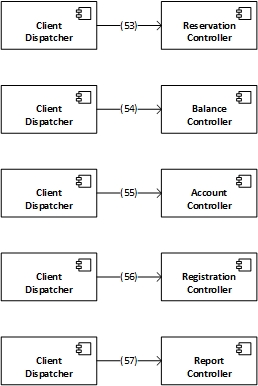
\includegraphics[scale=1]{CustomerDispatcher/Dispatcher_Integration}
\end{figure}

This is the final integrated module
\begin{figure}[H]
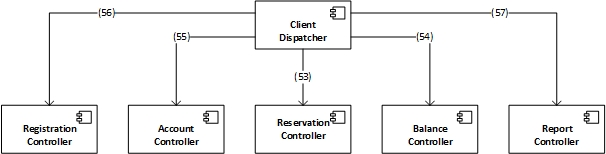
\includegraphics[scale=1]{CustomerDispatcher/Complete_Integration}
\end{figure}

\begin{Large}
\textbf{ClientDispatcher}
\end{Large}

We will integrate the ClientDispatcher with each one of the previously integrated modules
\begin{figure}[H]
\centering
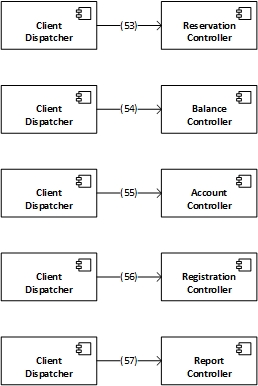
\includegraphics[scale=1]{CustomerDispatcher/Dispatcher_Integration}
\end{figure}

This is the final integrated module
\begin{figure}[H]
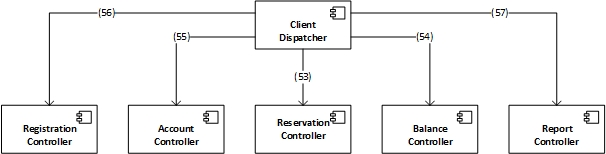
\includegraphics[scale=1]{CustomerDispatcher/Complete_Integration}
\end{figure}

\begin{Large}
\textbf{ClientDispatcher}
\end{Large}

We will integrate the ClientDispatcher with each one of the previously integrated modules
\begin{figure}[H]
\centering
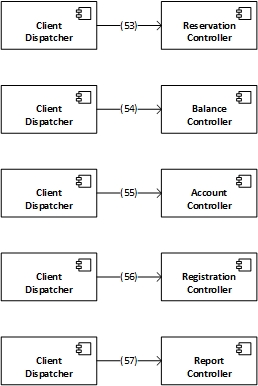
\includegraphics[scale=1]{CustomerDispatcher/Dispatcher_Integration}
\end{figure}

This is the final integrated module
\begin{figure}[H]
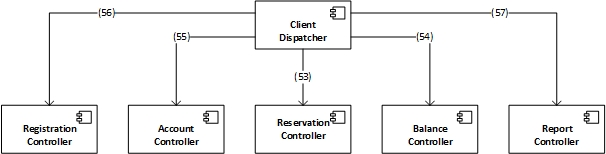
\includegraphics[scale=1]{CustomerDispatcher/Complete_Integration}
\end{figure}

\begin{Large}
\textbf{ClientDispatcher}
\end{Large}

We will integrate the ClientDispatcher with each one of the previously integrated modules
\begin{figure}[H]
\centering
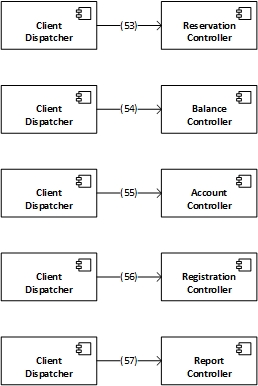
\includegraphics[scale=1]{CustomerDispatcher/Dispatcher_Integration}
\end{figure}

This is the final integrated module
\begin{figure}[H]
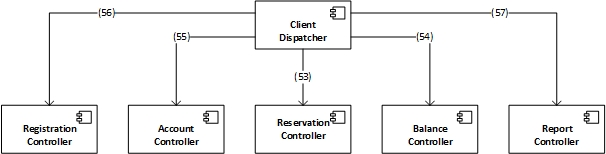
\includegraphics[scale=1]{CustomerDispatcher/Complete_Integration}
\end{figure}

\begin{Large}
\textbf{ClientDispatcher}
\end{Large}

We will integrate the ClientDispatcher with each one of the previously integrated modules
\begin{figure}[H]
\centering
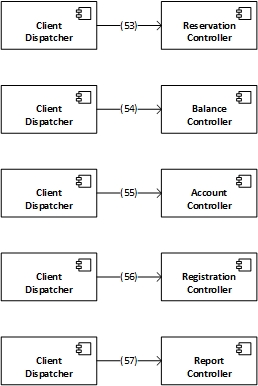
\includegraphics[scale=1]{CustomerDispatcher/Dispatcher_Integration}
\end{figure}

This is the final integrated module
\begin{figure}[H]
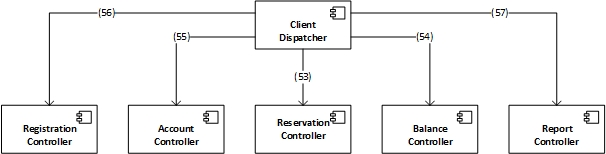
\includegraphics[scale=1]{CustomerDispatcher/Complete_Integration}
\end{figure}

\begin{Large}
\textbf{ClientDispatcher}
\end{Large}

We will integrate the ClientDispatcher with each one of the previously integrated modules
\begin{figure}[H]
\centering
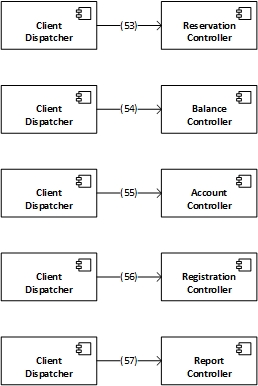
\includegraphics[scale=1]{CustomerDispatcher/Dispatcher_Integration}
\end{figure}

This is the final integrated module
\begin{figure}[H]
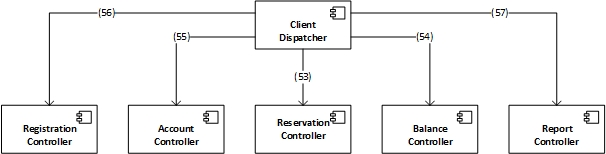
\includegraphics[scale=1]{CustomerDispatcher/Complete_Integration}
\end{figure}